%% This is an example first chapter.  You should put chapter/appendix that you
%% write into a separate file, and add a line \include{yourfilename} to
%% main.tex, where `yourfilename.tex' is the name of the chapter/appendix file.
%% You can process specific files by typing their names in at the 
%% \files=
%% prompt when you run the file main.tex through LaTeX.
\chapter{Application of DEnHKF to Hydrologic Model}

\section{daWUAPhydroengine}

The hydrologic model is used to test the viability of the DEnHKF method. The hydrologic model takes streamflow parameters, subbasin parameters, precipitation, minimum temperatures, and maximum temperatures as inputs and outputs streamflow data along with some additional states such as snow water equivalent. The hydrologic model was designed to be implemented in any geographic location. For this study it was utilized to model streamflows throughout the state of Montana.

\begin{table}[]
\caption{States} 
\begin{tabular}{lll}
State ($x$) & Purpose                              & Dimensions  \\ \hline
streamflow  & Streamflow (in cumecs)               & 330   \\
swe         & Snow Water Equivalent  (in $mm^{3}$) & 45012
\end{tabular}
\label{tab:states}
\end{table}

For the purposes of this study configuring the hydrologic model to model streamflows throughout Montana is advantageous because it allows for the calibration of a very large number of spatially distributed, high dimensional parameters. These parameters can be expected to vary significantly across the entirety of Montana, a state which covers an area of 380,800 $km^{2}$, sports diverse terrain, and is comprised of 3 HUC4 zones.

\subsection{Input Data}

The hydrologic model takes rasterized precipitation data and temperature data from meteorological databases as input. This data can be utilized as forcing data in the ensemble kalman filter framework.
\begin{table}[]
\caption{Forcing Data} 
\begin{tabular}{lll}
Forcing Data ($u$) & Purpose                          & Dimensions \\ \hline
tempmin          & Lowest temperature for timestep  & 45012 \\
tempmax          & Highest temperature for timestep & 45012 \\
precipitation      & Amount of rainfall for timestep & 45012 
\end{tabular}
\label{tab:u_params}
\end{table}

\subsection{Calibrated Parameters}

The hydrologic model utilizes a HBV rainfall-runoff component and a Muskingum-Cunge routing component. The HBV component includes a precipitation and snowpack process that utilizes the empirical parameter $ddf$ (degree day factor), a soil process that utilizes the empirical parameters $aet\_lp$, $soil\_beta$, and $soil\_max\_wat$ (evapo-transpiration, immediate runoff, and topsoil storage capacity), and a runoff generation process that utilizes the empirical parameters $ck0$, $ck1$, $ck2$, $hl1$, and $perc$, all of which control various aspects of groundwater percolation and runoff. The Muskingum-Cunge routing component utilizes $e$ and $K$, which control wave dispersion and wave celerity respectively. To learn more about the hydrologic model, its algorithms, and the parameters that control it refer to \autoref{chap:daWUAPhydroengine}.

\begin{table}[]
\caption{Calibrated Parameters} 
\begin{tabular}{lll}
Parameter ($\theta$) & Purpose                                                    & Dimensions  \\ \hline
$ddf$                  & Degree Day Factor                                        & 331 \\
$aet\_lp$              & Potential Evapo-Transpiration                                                      & 331 \\
$soil\_beta$           & Portion of ponded water that goes into soil storage & 331 \\
$soil\_max\_wat$       & Soil compartment maximum water capacity & 331 \\
$ck0$       & Immediate runoff & 330 \\
$ck1$      & Fast runoff & 330 \\
$ck2$       & Groundwater runoff & 330 \\
$hl1$       & Groundwater water storage threshold & 330 \\
$perc$       & Groundwater peculation & 330 \\
$K$       & Wave celerity & 330 \\
$e$       & Wave dispersion & 330 \\
\end{tabular}
\label{tab:t_params}
\end{table}



\section{Observation Data}

A Kalman Filter relies on one or more observed states for correction. Accordingly, observations were obtained for streamflows across Montana and snowfall across Montana. For streamflow, USGS streamflow data was collected at 86 sites. Each observed site was paired with the closest simulated stream outlet within a 2.5 mile cutoff. For snowfall, SNOWTEL sites monitored by the Natural Resources Conservation Service (NRCS) were used \ref{fig:stations}. 90 stations were chosen and matched to specific pixels in the hydrologic model's raster files.


\begin{table}[]
\caption{Observations} 
\begin{tabular}{lll}
Observed State ($x$) & Source                              & Dimensions  \\ \hline
streamflow  & USGS & 82   \\
swe         & NRCS & 90
\end{tabular}
\label{tab:obs}
\end{table}

\begin{figure}[h]
    \centering
    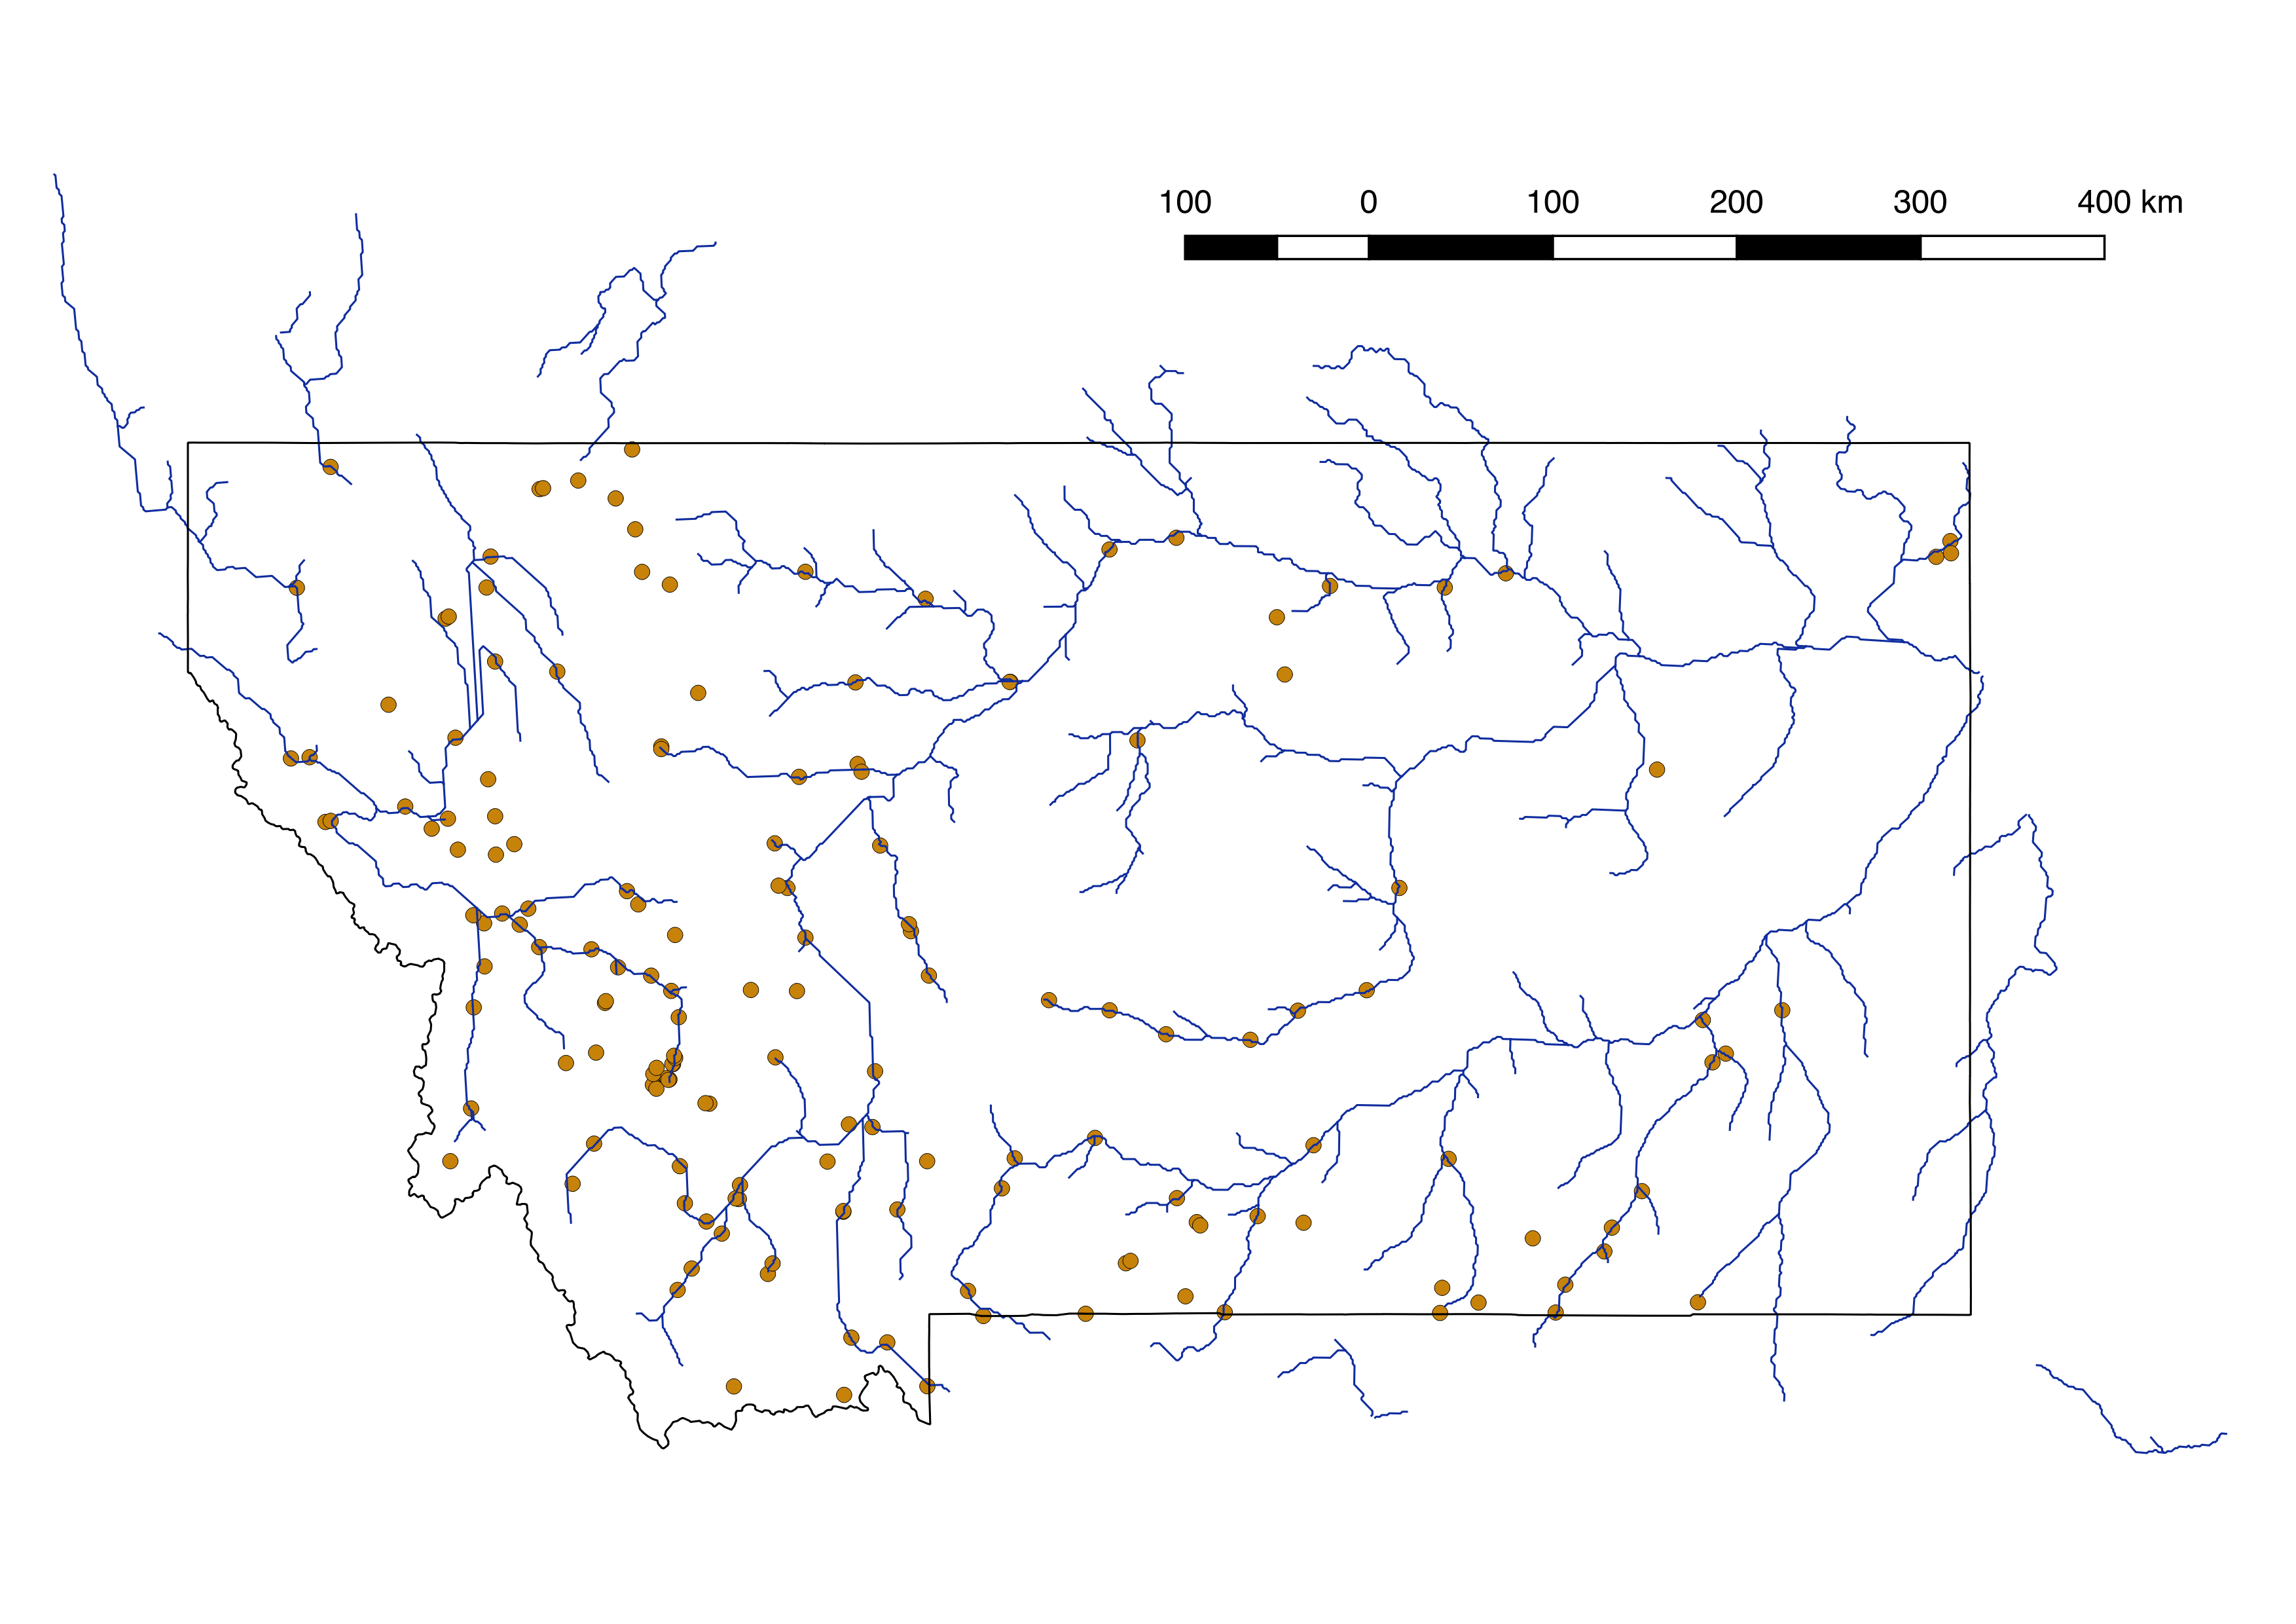
\includegraphics[width=0.95\textwidth]{stations}
    \caption{all SWE stations plotted against modeled streamflows}
    \label{fig:stations}
\end{figure}

\section{Catchment Data and Hierarchical Groups}

The hydrologic model uses HUC8 data to separate Montana into 330 watersheds \ref{fig:huc8}. Each watershed is associated with one of each type of parameter from Table \ref{tab:t_params}. These 330 watersheds fall into 3 larger HUC4 zones that were utilized to classify each watershed into one of 3 hierarchical zones \ref{fig:huc4}.

\begin{figure}[h]
    \centering
    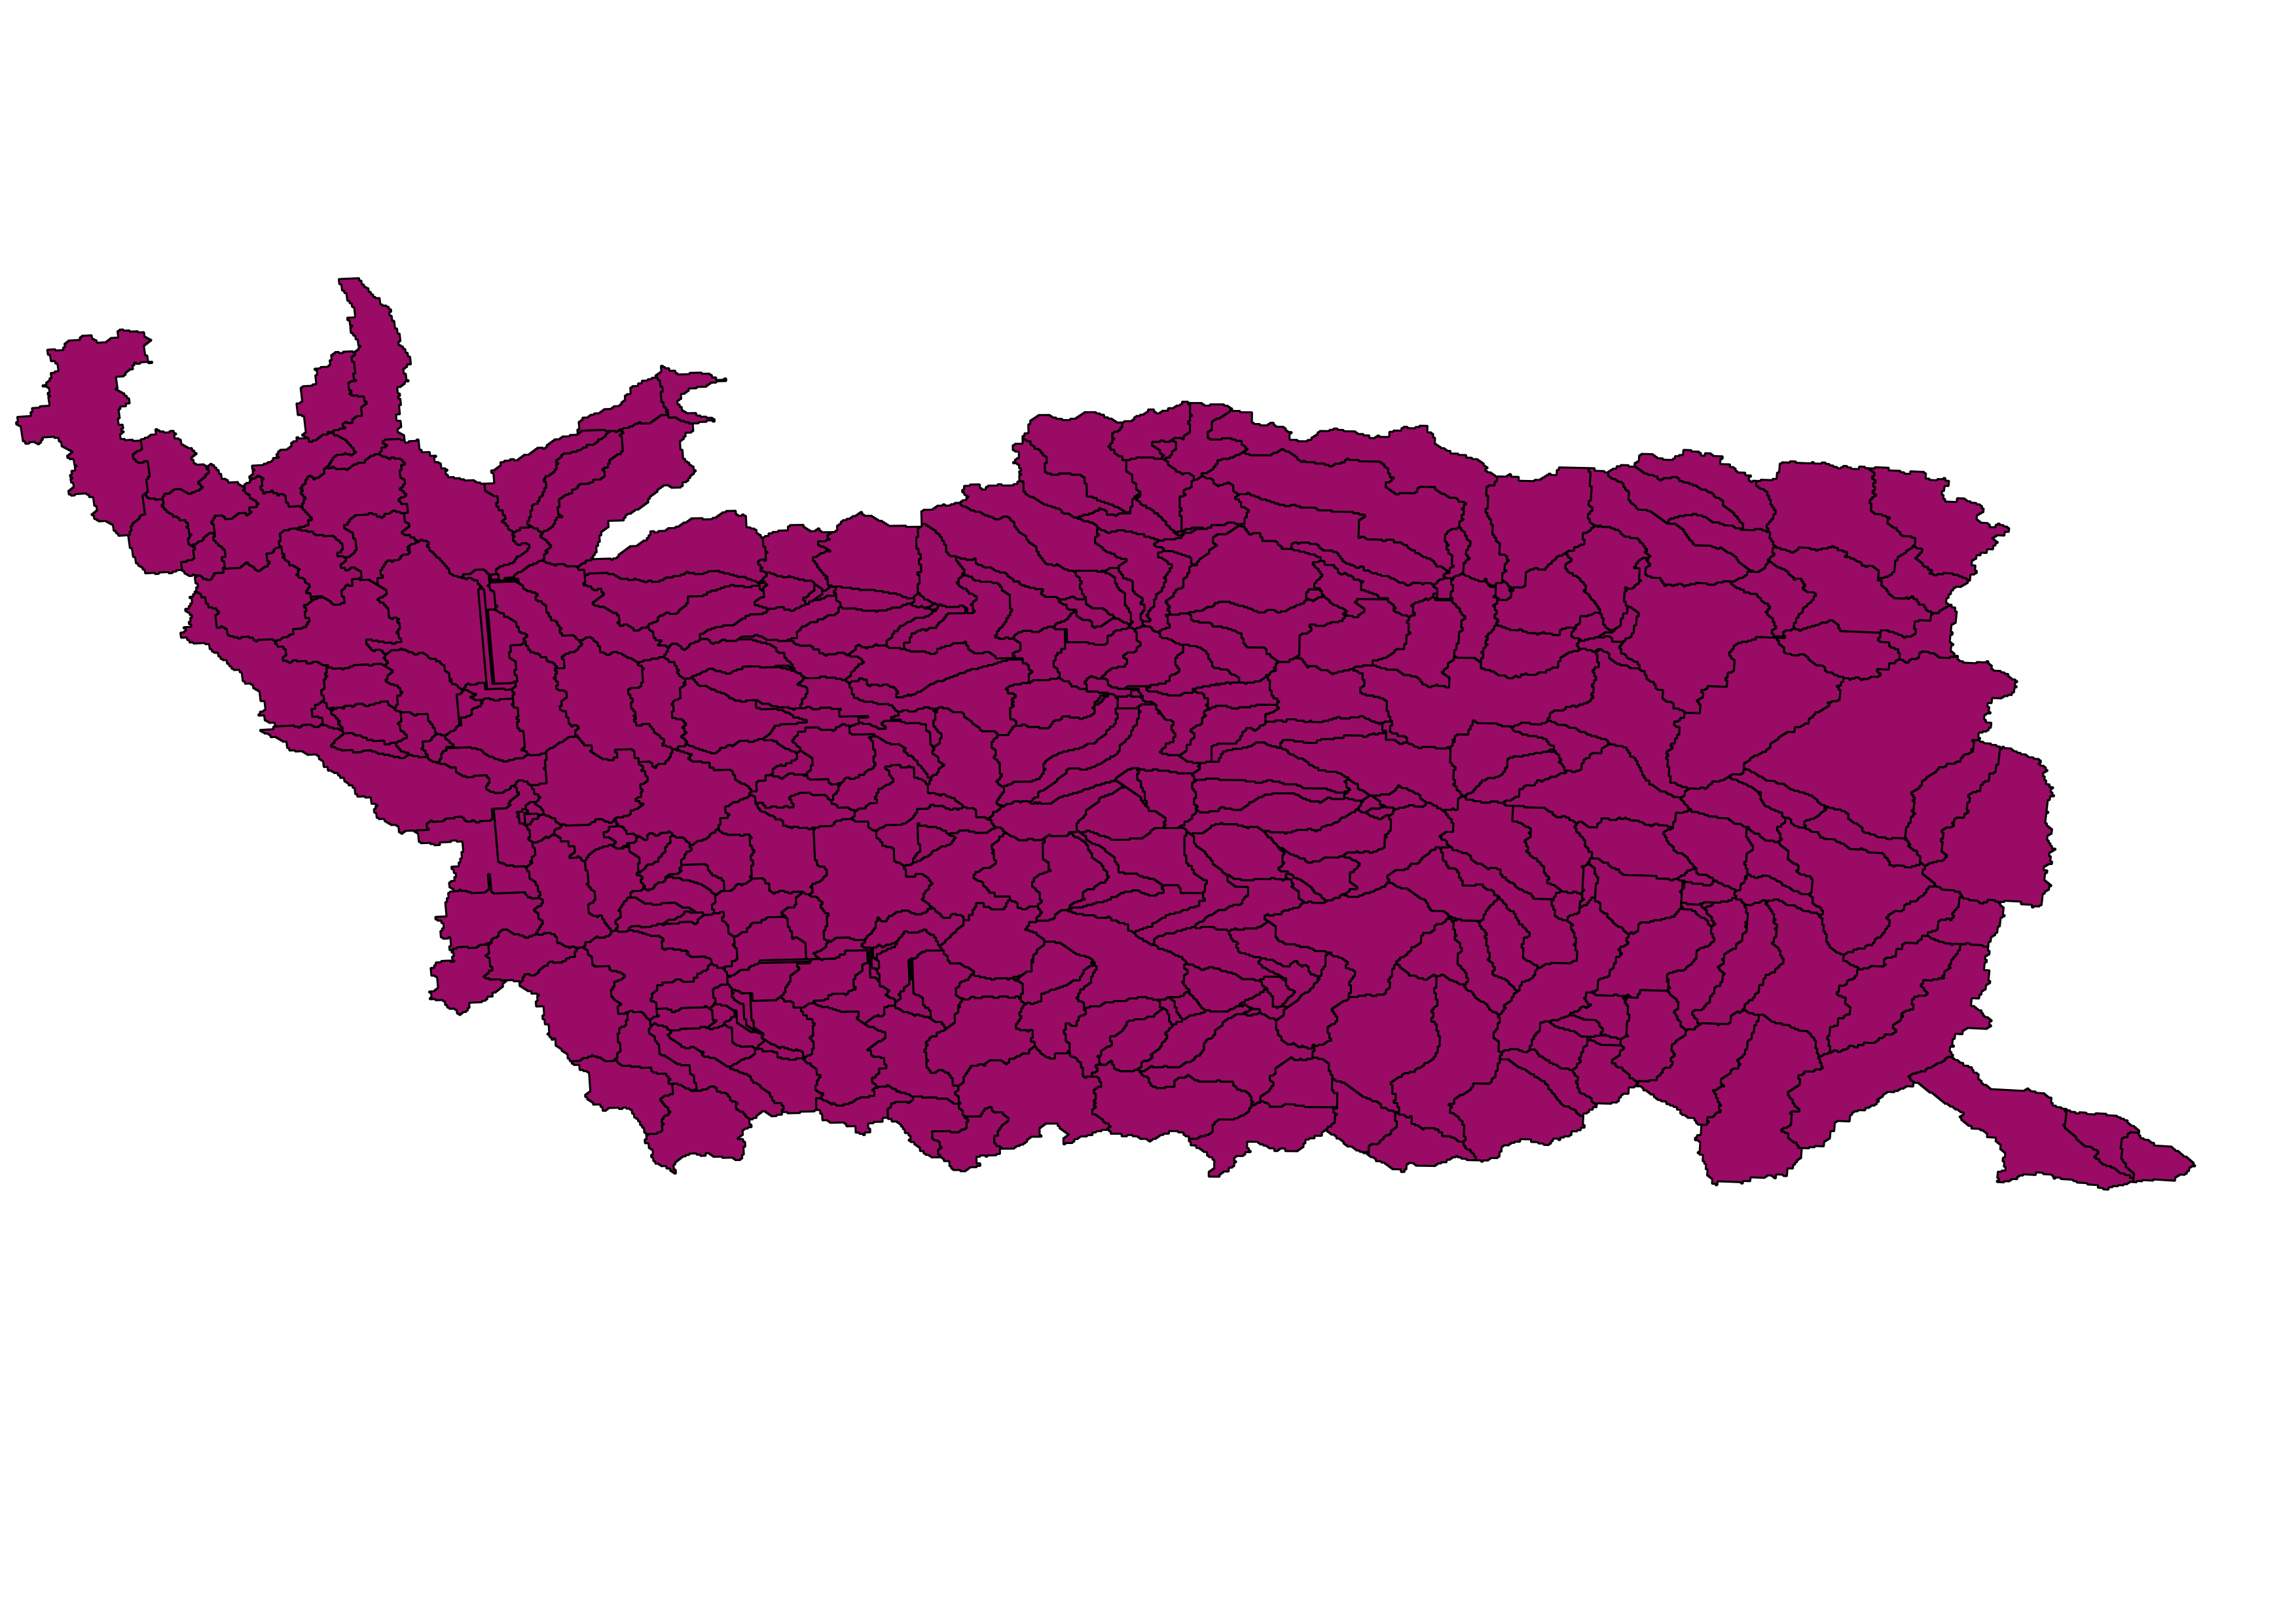
\includegraphics[width=0.95\textwidth]{huc8}
    \caption{Subbasins - HUC8 polygons}
    \label{fig:huc8}
\end{figure}

\begin{figure}[h]
    \centering
    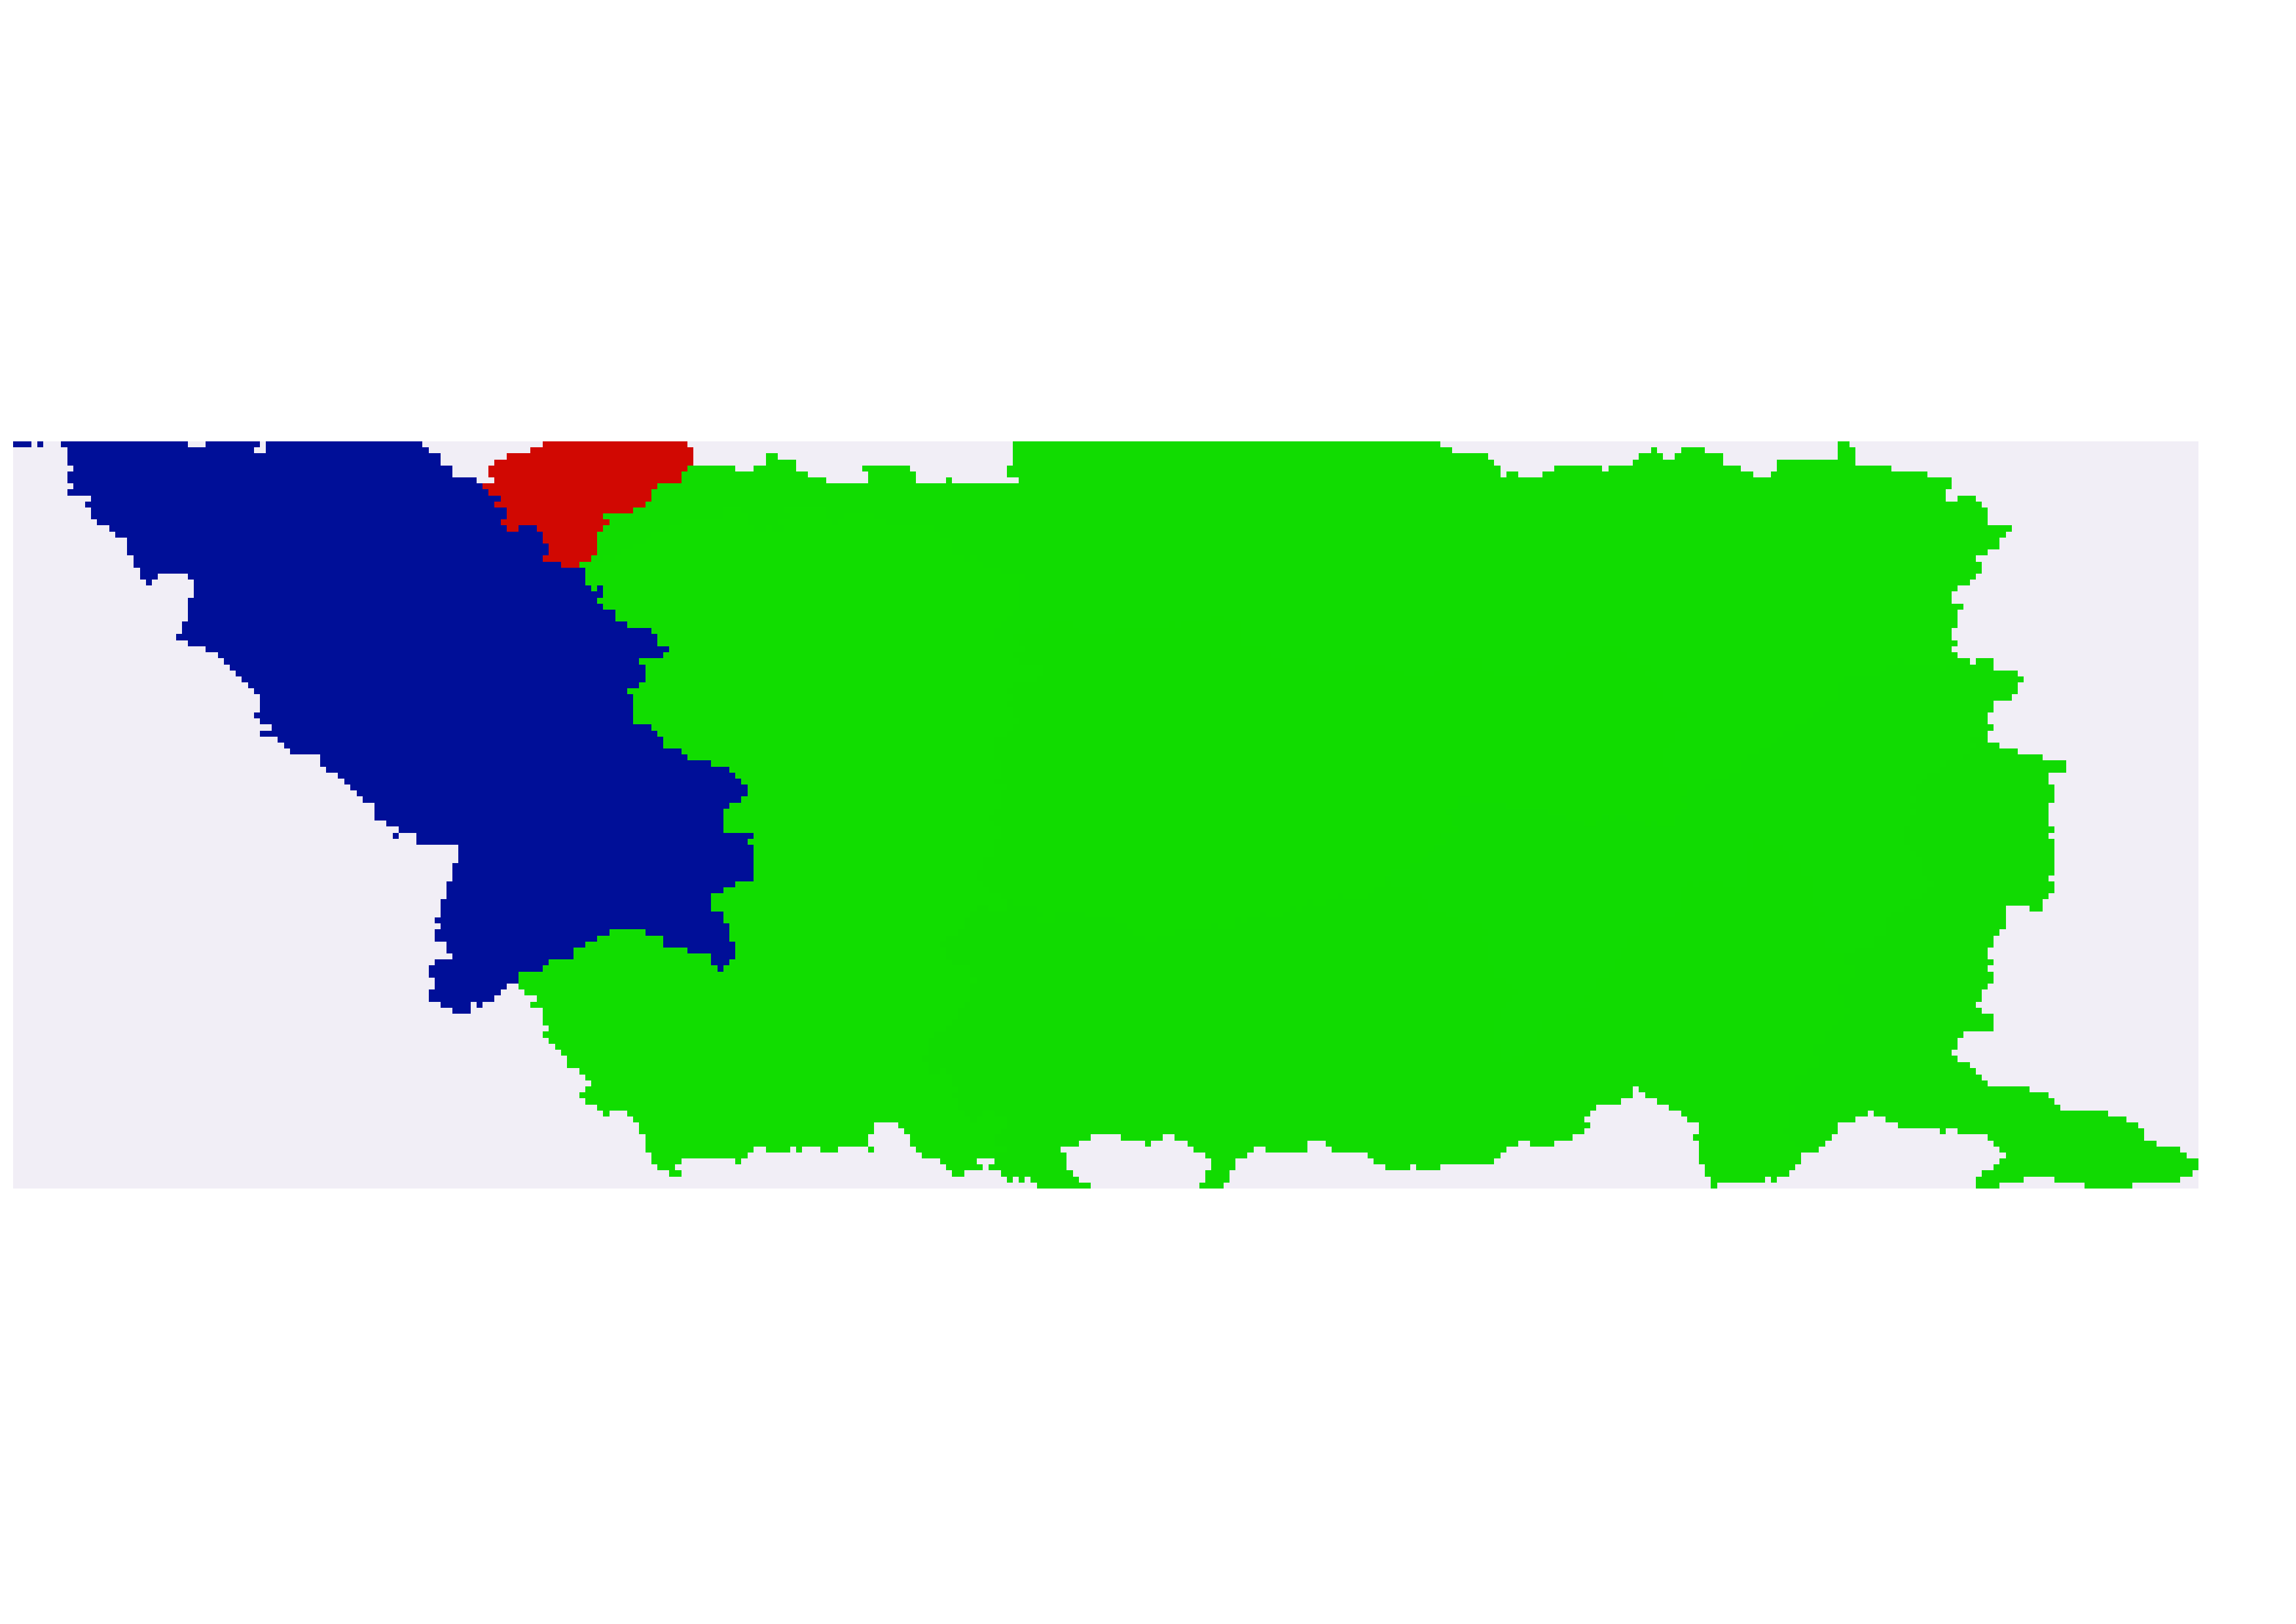
\includegraphics[width=0.95\textwidth]{huc4}
    \caption{Montana's 3 HUC4 zones rendered onto the raster grid.}
    \label{fig:huc4}
\end{figure}
